\documentclass[11pt]{article}%文档类型

\usepackage[a4paper]{geometry}
\geometry{left=2.0cm,right=2.0cm,top=2.5cm,bottom=2.5cm}

%使用如下的宏包
\usepackage{ctex}
\usepackage{amsmath,amsfonts,graphicx,amssymb,bm,amsthm}
\usepackage{algorithm,algorithmicx}
\usepackage[noend]{algpseudocode}
\usepackage{fancyhdr}
\usepackage{fancyvrb}
\usepackage{color}
\usepackage[most]{tcolorbox}
\usepackage{subfigure}
\usepackage{xhfill}
\usepackage{url}
\usepackage[colorlinks=true,linkcolor=red]{hyperref}

\newcommand{\vrb}[1]{\fcolorbox{green}{yellow}{#1}}
%\newcommand{\vrb}[1]{\fcolorbox{yellow!10!white}{yellow!10!white}{#1}}

\title{盒子与浮动体}
\author{王新鹏\footnote{\url{wangxinpeng16@mails.ucas.ac.cn}}  \quad  施春江\footnote{\url{shichunjiang16@mails.ucas.ac.cn}}}

\begin{document}
\maketitle

\section{盒子}

盒子是 排版的基础单元。\LaTeX 的输出页面本身就是一个大盒子,这个大盒子内部由很多的小盒子构成,每一行内容都是一个盒子,页面就是盒子套盒子的大盒子。

每个盒子的左侧均有一参考点 (Reference point)。盒子的基线(baseline)是通过参考点的一条水平线。当 \LaTeX 排版时,位于同一行盒子的参考点将被从左到右的排成一条直线,称为当前基线(current baseline),并使它与盒子的基线对齐。每个对象的参考点都被放置于当前基线上。

描述盒子主要是三个参数分别是高度,深度,宽度。高度是参考点到盒子顶部的距离,深度是参考点到盒子底部的距离,宽度则是盒子的宽度。\LaTeX 提供了一些实用的命令让我们生成一些有用的盒子。
\subsection{水平盒子}
水平盒子即水平对齐的盒子。
\subsubsection{mbox 和 fbox 命令}

\begin{verbatim}
\mbox{文本} 和 \makebox[宽度][位置参数]{文本}
\fbox{文本} 和 \framebox[宽度][位置参数]{文本}
\end{verbatim}

左侧两条命令生成一个简单水平盒子,其宽度恰好是在\{ \}中给出的文本的宽度。  \vrb{fbox} 和 \vrb{framebox} 有外框,除此以外和前者相同。

\emph{例子}:
    \begin{verbatim}    
        |\mbox{Test some words.}|\\ 
        |\makebox[10em]{Test some words.}|\\ 
        |\makebox[10em][l]{Test some words.}|\\ 
        |\makebox[10em][r]{Test some words.}|\\ 
        |\makebox[10em][s]{Test some words.}|
    \end{verbatim}

\fbox{
    \begin{minipage}[c]{18em}%
        |\mbox{Test some words.}|\\ 
        |\makebox[10em]{Test some words.}|\\ 
        |\makebox[10em][l]{Test some words.}|\\ 
        |\makebox[10em][r]{Test some words.}|\\ 
        |\makebox[10em][s]{Test some words.}|
    \end{minipage}}




\emph{例子}:
    \begin{verbatim}
        |\fbox{Test some words.}|\\ 
        |\framebox[10em]{Test some words.}|\\ 
        |\framebox[10em][l]{Test some words.}|\\ 
        |\framebox[10em][r]{Test some words.}|\\ 
        |\framebox[10em][s]{Test some words.}|\\
        |\fcolorbox{green}{red}{Test some words.}|
    \end{verbatim}

\fbox{
    \begin{minipage}[c]{18em}%
        |\fbox{Test some words.}|\\ 
        |\framebox[10em]{Test some words.}|\\ 
        |\framebox[10em][l]{Test some words.}|\\ 
        |\framebox[10em][r]{Test some words.}|\\ 
        |\framebox[10em][s]{Test some words.}|\\
        |\fcolorbox{green}{red}{Test some words.}|
    \end{minipage}
}

    
右面两条命令生成由可省的长度参数来预先确定宽度的盒子文本的自然宽度要比所定义的宽度大的时候,就会出现突出。位置参数可以取居中 \vrb{c}(默认)、左对齐 \vrb{l}、右对齐 \vrb{r} 和分散对齐 \vrb{s}。

|\mbox{Test some words.}|\\

\subsubsection{makebox 命令}
 \vrb{makebox} 命令,可在picture环境中生成一个居中的或者左右对齐的文本,也可以使部分文本重叠,如
\begin{verbatim}
\makebox[0pt][l]{/}S
\end{verbatim}
输出结果是\makebox[0pt][l]{/}S

\makebox[0pt][l]{/}哈


\subsubsection{边框和调整}
\begin{verbatim}
\framebox[10em][r]{Test box}\\[1ex]
\setlength{\fboxrule}{1.6pt}
\setlength{\fboxsep}{1em}
\framebox[10em][r]{Test box}
\end{verbatim}
\vrb{setlength} 命令可以调整边框的宽度 \vrb{fboxrule} 和内边距\vrb{fboxsep},注意长度需要带单位。
宽度单位有 \vrb{cm}/\vrb{in}/\vrb{em},笔者比较喜欢宽度单位 \vrb{textwidth}
\subsubsection{保存和调用}
\begin{verbatim}
\newsavebox{\boxname}
\sbox{\boxname}{文本} or \savebox[宽度][位置]{文本}
\usebox{\boxname}
\end{verbatim}
以上三条命令可以初始化,保存和调用已有的盒子。

\subsubsection{盒子的竖直移位}
\begin{verbatim}
\raisebox{上移量}[高度][深度]{文本}
\end{verbatim}

\subsection{垂直盒子}
垂直盒子即垂直对齐的盒子, \LaTeX 提供了两种方式:
\begin{verbatim}
\parbox[整体位置参数][高度][内部位置参数]{宽度}{文本}
\begin{minipage}[整体位置参数][高度][内部位置参数]{宽度}
. . .
\end{minipage}
\end{verbatim}
和水平盒子不同,内部位置参数接受的选项是顶部t、底部b、居中c 和分散对齐s。

如果在 \vrb{minipage} 里使用 \vrb{footnote} 命令,生成的脚注会出现在盒子底部,编号是独立的,
并且使用小写字母编号。这也是 \vrb{minipage} 环境之被称为“迷你页”(Mini-page)的原因。而在
parbox 里无法正常使用 \vrb{footnote} 命令,只能在盒子里使用 \vrb{footnotemark},在盒子外使用 \vrb{footnotetext}。

\emph{例子}:
    \begin{verbatim}
        这是一个例子。
        \footnote{例子脚注来自 minipage。}
    \end{verbatim}

\fbox{
    \begin{minipage}[c]{18em}%
        这是一个例子。
        \footnote{例子脚注来自 minipage。}
    \end{minipage}
}

\subsection{标尺盒子}
rule 命令用来画一个实心的矩形盒子,也可适当调整以用来画线。
\begin{verbatim}
\rule[位置浮动]{宽度}{高度}
A \rule[-.4pt]{3em}{.4pt} line.
\end{verbatim}
也可以生成一个宽度为零的标尺盒子,这样得到一个不可见的具有给定高度的盒子,如此的构造称为一个支撑,如此可以强迫所在的水平盒子具有不同于其所包含内容需要的高度和深度.

\subsubsection{推荐: tcolorbox package}
\emph{例子}:

\begin{verbatim}
    \begin{tcolorbox}[ams align,colback=yellow!10!white,colframe=red!50!black]
        \sum\limits_{n=1}^{\infty} \frac{1}{n} &= \infty.\\
        \int x^2 ~\text{d}x &= \frac13 x^3 + c.
    \end{tcolorbox}
\end{verbatim}

\begin{tcolorbox}[ams align,colback=yellow!10!white,colframe=red!50!black]
    \sum\limits_{n=1}^{\infty} \frac{1}{n} &= \infty.\\
    \int x^2 ~\text{d}x &= \frac13 x^3 + c.\\
    说:你是猪!
\end{tcolorbox}
    

\newpage
\section{浮动体}
浮动体包括两个重要内容:\textbf{图片(figure)}和\textbf{表格(table)}。
\LaTeX 将它们加入了浮动体的机制,令其中大块的内容可以脱离上下文,放置在合适的位置。理论上以在任何一个浮动体里放置文字、公式、表格、图片等等任意内容。虽然说浮动是目的,但是笔者在排版时经常因为图片放不到合适的位置而取消 \vrb{figure} 和 \vrb{table} 的浮动,这里自己见仁见智。

\section{table}
\subsection{table 环境用法}
\begin{verbatim}
    \begin{table}[位置参数]
        放置文字、公式、表格、图片等等任意内容。
    \end{table}
\end{verbatim}

位置参数用一系列符号用来表示浮动体允许排版的位置,如 hbp 允许浮动体排版在当前位置、底部或者单独成页。table 和 figure 浮动体的默认设置为 tbp。

\begin{table}[htbp]
    \centering
    \caption{浮动体的位置参数。}
    \begin{tabular}{cc}
        \hline
        \textbf{参数}     &\textbf{含义}\\ \hline
        h       &当前位置(代码所处的上下文)\\
        t       &顶部\\
        b       &底部\\
        p       &单独成页\\
        !       &在决定位置时忽视限制\\
        \hline\hline
    \end{tabular}
\end{table}

注 1:排版位置的选取与参数里符号的顺序无关,L A TEX 总是以 h-t-b-p 的优先级顺序决定浮动体位置。也就是说 [!htp] 和 [ph!t] 没有区别。
注 2:限制包括浮动体个数(除单独成页外,默认每页不超过 3 个浮动体,其中顶部不超过 2 个,底部不超过 1 个)以及浮动体空间占页面的百分比(默认顶部不超过 70\%,底部不超过 30\%)。

举个\emph{例子}:
\begin{verbatim}
    \begin{table}[htbp]%[!htbp]  %按经验建议htbp的参数
        \centering
        \caption{浮动体的位置参数。}  %标题
        \begin{tabular}{cc}  %{c|c}  %c是对齐参数
            \hline
            参数     &含义\\ \hline
            h       &当前位置(代码所处的上下文)\\
            t       &顶部\\
            b       &底部\\
            p       &单独成页\\
            !       &在决定位置时忽视限制\\
            \hline\hline
        \end{tabular}
    \end{table}
\end{verbatim}


\textbf{笔者建议}:根据使用经验,使用如 \fcolorbox{yellow}{yellow}{Excel2Latex} / \fcolorbox{yellow}{yellow}{Cal2LaTeX} 的 插件/宏,节省从数据文件格式导入到 \LaTeX 的时间,尤其是有大量单元格合并的表格。

%\subsection{\vrb{table}的调整}
%来不及写了QAQ

\subsection{图片(figure)}
\subsubsection{单个图片}
\begin{verbatim}
    \begin{figure}[htbp]
        \centering %图片在页面居中位置
        \includegraphics[width=0.85\textwidth]{文件路径}
        \caption{标题}   
        \label{标签,不显示,方便上下文引用:\ref{标签}}
    \end{figure}
\end{verbatim}

\subsubsection{多个图片的排版}
直接排版,如果图片比例不一致就无法对齐。
\begin{verbatim}
    \begin{figure}[htbp]
        \centering
        \includegraphics[width=...]{...}
        \qquad %分隔,不加亦可
        \includegraphics[width=...]{...} \\[..pt] %换行
        \includegraphics[width=...]{...}
        \caption{...}
    \end{figure}
\end{verbatim}

\begin{figure}[htbp]
    \centering
    
\includegraphics[width=0.45\textwidth]{Img/ucaslogo}
    \qquad %分隔左右两个图
    \includegraphics[width=0.45\textwidth]{Img/ucas_logo} \\[5pt] %换行
    
\includegraphics[width=0.45\textwidth]{Img/ucaslogo}
    \caption{标题:ucaslogo。}
\end{figure}

\quad\xdotfill{2pt}[blue] \vrb{minipage}\xdotfill{2pt}[blue] \quad

使用\vrb{minipage}环境,可以在每一个图下分开加入标题:
\begin{verbatim}
    \begin{figure}[htbp]
        \begin{minipage}[t]{0.5\linewidth}
            \centering
            \includegraphics[width=1.0\textwidth]{图片路径}
            \caption{子图1}
        \end{minipage}%
        \begin{minipage}[h]{0.5\linewidth}
            \centering
            \includegraphics[width=1.0\textwidth]{图片路径}
            \caption{子图2}
        \end{minipage} \\
        \begin{minipage}[t]{0.5\linewidth}
            \centering
            \includegraphics[width=0.5\textwidth]{图片路径}
            \caption{子图3}
        \end{minipage}
    \end{figure}
\end{verbatim}

\begin{figure}[htbp]
    \begin{minipage}[t]{0.5\linewidth}
        \centering
        
\includegraphics[width=1.0\textwidth]{Img/ucaslogo}
        \caption{子图1}
    \end{minipage}%
    \begin{minipage}[h]{0.5\linewidth}
        \centering
        \includegraphics[width=1.0\textwidth]{Img/ucas_logo}
        \caption{子图2}
    \end{minipage} \\
    \begin{minipage}[t]{0.5\linewidth}
        \centering
        
\includegraphics[width=0.5\textwidth]{Img/ucaslogo}
        \caption{子图3}
    \end{minipage}
\end{figure}

\quad\xdotfill{2pt}[blue] \vrb{subfigure}\xdotfill{2pt}[blue] \quad

更近一步,在科学论文中使用子图常用 \fcolorbox{yellow}{yellow}{subfig} package 实现漂亮标准的子图排版, 命令为:
\begin{verbatim}
    \subfloat[...]{   %\label{} 这里可以加个标签
    \begin{minipage}{...}
        ...
    \end{minipage}
    }
\end{verbatim}

笔者之前使用的是\fcolorbox{yellow}{yellow}{subfigure}实现相同的功能,例如:


\begin{figure}[htbp]
    \centering 
    \subfigure[$C_{TT}$能谱.]{ 
        \label{fig:subfig:a} %% label for first subfigure 
        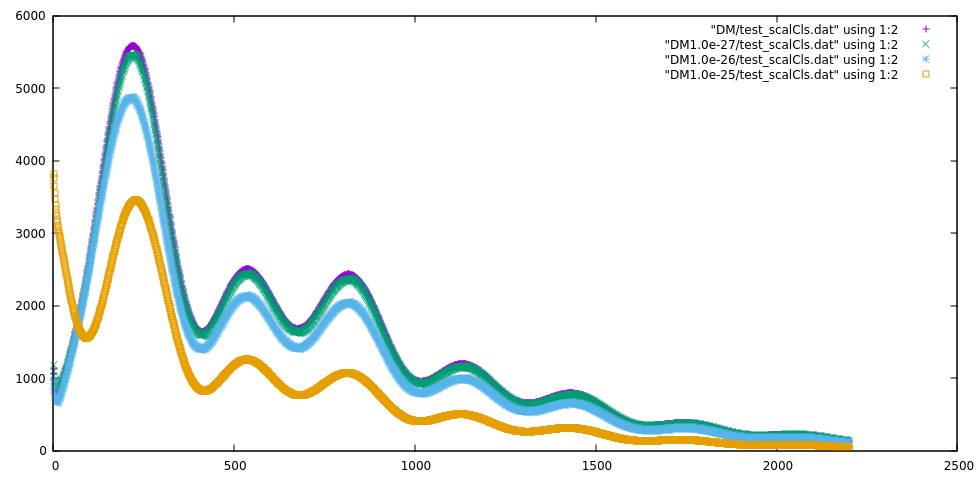
\includegraphics[width=0.4\textwidth]{Img/example1}} 
    \hspace{0.5in} 
    \subfigure[$C_{EE}$能谱.]{ 
        \label{fig:subfig:b} %% label for second subfigure 
        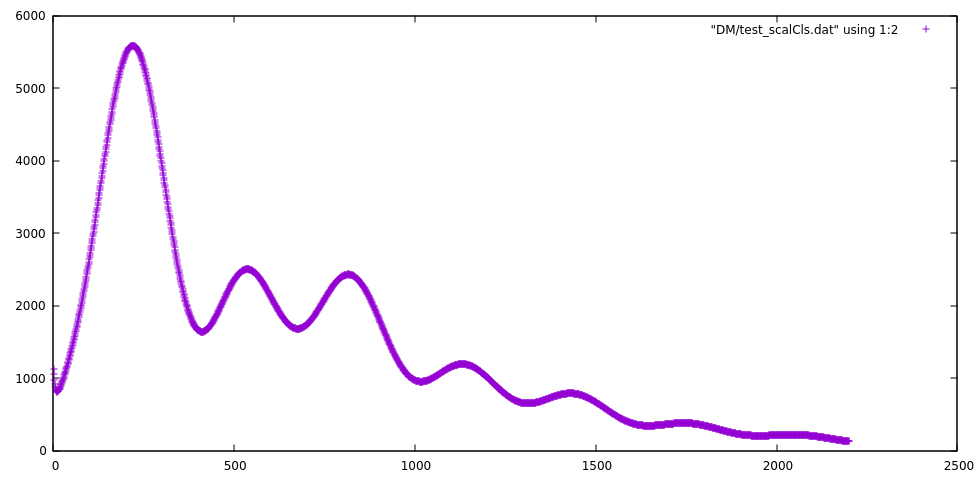
\includegraphics[width=0.4\textwidth]{Img/example2}}
    \\
    \subfigure[$C_{TE}$能谱.]{ 
        \label{fig:subfig:c} %% label for third subfigure 
        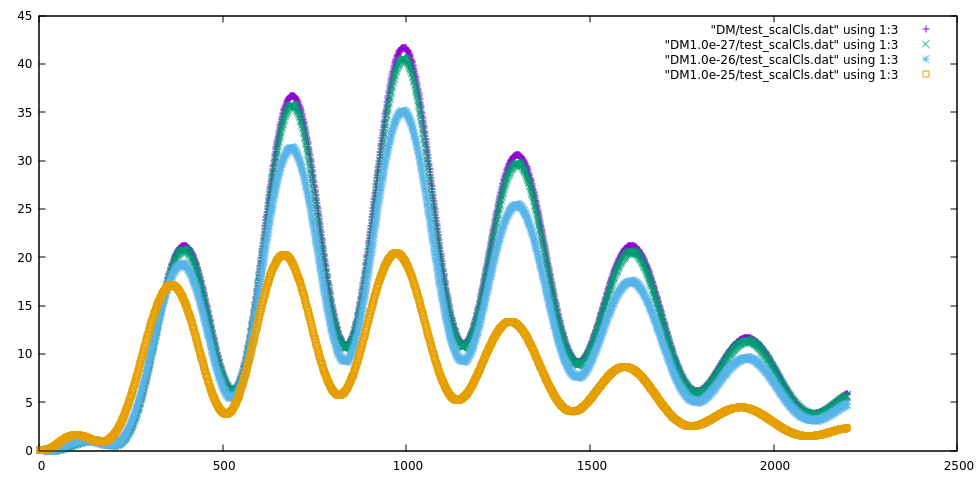
\includegraphics[width=0.4\textwidth]{Img/example3}} 
    \hspace{0.5in} 
    \subfigure[$C_{\Phi}$能谱.]{ 
        \label{fig:subfig:d} %% label for fourth subfigure 
        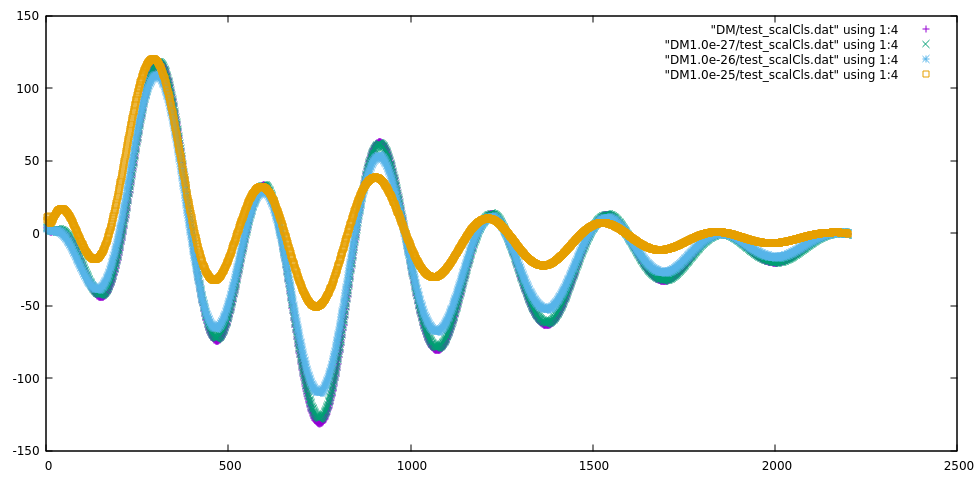
\includegraphics[width=0.4\textwidth]{Img/example4}}
    \caption{CMB两点相关函数.  添加了\vrb{label}实现应用: \ref{fig:subfig:a}为$C_{TT}$能谱.} 
    \label{fig:subfig} %% label for entire figure 
\end{figure}

\begin{verbatim}
\begin{figure}[htbp]
    \centering 
    \subfigure[这里是子图标题a]{ 
        \label{fig:subfig:a} %% label for first subfigure 
        \includegraphics[width=0.4\textwidth]{子图a路径}} 
    \hspace{0.5in} 
    \subfigure[这里是子图标题b]{ 
        \label{fig:subfig:b} %% label for second subfigure 
        \includegraphics[width=0.4\textwidth]{子图b路径}}
    \\
    \subfigure[这里是子图标题a]{ 
        \label{fig:subfig:a} %% label for third subfigure 
        \includegraphics[width=0.4\textwidth]{子图c路径}} 
    \hspace{0.5in} 
    \subfigure[这里是子图标题b]{ 
        \label{fig:subfig:b} %% label for fourth subfigure 
        \includegraphics[width=0.4\textwidth]{子图d路径}}
    \caption{Two Subfigures} 
    \label{fig:subfig} %% label for entire figure 
\end{figure}
\end{verbatim}

\section{参考文献}
内容参考\fcolorbox{yellow}{yellow}{lshort} / \fcolorbox{yellow}{yellow}{tcolorbox} / \fcolorbox{yellow}{yellow}{fancybox} / \fcolorbox{yellow}{yellow}{subfigure} 等package documentation。 

\end{document}